\documentclass[11pt]{beamer}
\usetheme{metropolis}
\usepackage[utf8]{inputenc}
\usepackage[english]{babel}
\usepackage[T1]{fontenc}
\usepackage{amsmath}
\usepackage{amsfonts}
\usepackage{amssymb}
\usepackage{bm}
\usepackage{subfig}
\usepackage{pgfplots}
\pgfplotsset{compat=newest}
%\usepackage{booktabs}
\newcommand{\Ex}{\mathbb{E}}
\newcommand{\Var}{\mathbb{V}\mathrm{ar}}
\newcommand{\Prob}{\mathbb{P}}
\DeclareMathOperator*{\argmin}{arg\,min}
\DeclareMathOperator*{\argmax}{arg\,max}
\graphicspath{{./Figures/}}

\title{Parameter control in the presence of uncertainties}
\author{{\large Victor Trappler } \\ Supervisors: Elise Arnaud, Laurent Debreu, Arthur Vidard}
\institute{AIRSEA (Inria)-- LJK \\
 \begin{center}

\includegraphics[scale=0.20]{INRIA_SCIENTIFIQUE_UK_CMJN}

\includegraphics[scale=0.20]{ljk}
\end{center}
}
\date{\today}
\setcounter{tocdepth}{1}

\begin{document}
\frame{
\maketitle
}

\section{Introduction}
\frame{
\frametitle{Bottom friction}
\begin{itemize}
\item The friction of the ocean bed has an influence on the water circulation
\item Depends on the type and/or characteristic length of the asperities 
\item Subgrid phenomenon
\end{itemize}
\begin{center}
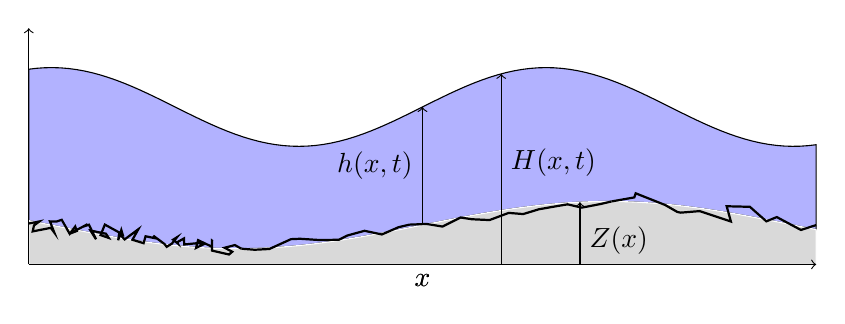
\begin{tikzpicture}
\usetikzlibrary{decorations.pathmorphing}

\definecolor{copper}{rgb}{0.69, 0.25, 0.21}
\definecolor{tin}{rgb}{0.7, 0.7, 0.7}

\tikzset{
  rugous1/.style = {black, thick,
    decoration={random steps,segment length=0.05cm,amplitude=.1cm}
  },
}
\tikzset{
  rugous2/.style = {black, thick,
    decoration={random steps,segment length=0.2cm,amplitude=.05cm}
  },
}
\tikzset{
  rugous3/.style = {black, thick,
    decoration={random steps,segment length=0.2cm,amplitude=.15cm}
  },
}

\filldraw [fill = blue!30]
   plot [samples = 100,domain = -5:5] (\x, {0.5*sin(\x r) + 2} )
-- plot [samples = 100,domain = 5:-5] (\x, {0.3*sin(\x/1.5 r)+0.5})
-- cycle;

\filldraw[fill = gray!30, draw = white]
   plot [samples = 100,domain = -5:5] (\x, {0.3*sin(\x/1.5 r)+0.5})
-- plot [samples = 100,domain = 5:-5] (\x, 0)
-- cycle;

\draw[rugous1, decorate](-5,0.52) -- (-2.3,0.2);
\draw[rugous2, decorate](-2.3,0.2) -- (2.4,0.8);
\draw[rugous3, decorate](2.4,0.8) -- (5,0.5);

\draw[->] (-5,0) -- (5,0);
\draw (0,0) node[below] {$x$};



\draw[->] (-5,0) -- (-5,3);

\draw[->] (0,0.5) -- (0,2);
\draw (0, 1.25) node[left] {$h(x,t)$} ;
\draw (0,0) node[below] {$x$};
\draw[->] (2,0) -- (2,{0.3*sin(2/1.5 r)+0.5});
\draw (2, 0.3) node[right] {$Z(x)$} ;
\draw[->] (1,0) -- (1,{0.5*sin(1 r)+2});
\draw (1, 1.3) node[right] {$H(x,t)$} ;
\end{tikzpicture}
\end{center}
}
\frame{
\frametitle{Outline}
\tableofcontents
}
\section{Deterministic problem}
\frame[t]{
\frametitle{Computer code : the Shallow Water Equations}
\begin{itemize}
	\item[Input] 
	\begin{itemize}
		\item $\bm{K}$: Bottom friction (spatially distributed)
		\item $\bm{X}_e$: Environmental variables (fixed and known)
	\end{itemize}
	\item[Output] \begin{itemize}
	\item $W(K) = \{W_i^n(K)\}_{i,n}$, where $W_i^n(K) = [h_i^n(K) \quad q_i^n(K)]^T$\\ for $0 \leq i \leq N_x$ and $0 \leq n \leq N_t$
	\end{itemize}
\end{itemize}
\vfill
\only<1>{\tikzstyle{block} = [rectangle, draw, fill=blue!20, 
     text centered, minimum width=1cm]

\tikzstyle{block2} = [rectangle, draw, fill=green!20, 
     text centered, rounded corners, minimum width=1cm]

\tikzstyle{LHS}=[rectangle, draw, text centered]

\begin{tikzpicture}[node distance=3cm]

\node [align = center] at (0,0) (input) {Control variable \\$K \in \mathcal{K}$};
%\node [align = center] at (4,1.5) (envir) {Environmental variables \\$\bm{u} \in \mathcal{U}$ fixed};
\node [align = center] at (4,1.5) (envir) {Environmental variables \\$\bm{x}_e \in \mathbb{X}$ fixed};

\node[block] at (4,0)(code){Direct Simulation};

\node[align = center] at (8,0) (output) {$W(K)$}; %\\ $\Rightarrow j(K)$};

\draw[->] (input) -- (code);
\draw[->] (envir) -- (code);
\draw[->] (code) -- (output);

\end{tikzpicture}}
\only<2>{\usetikzlibrary{positioning}
% \tikzstyle{block} = [rectangle, draw, fill=blue!30, 
%     text centered, minimum width=3em] 
 \tikzstyle{block} = [rectangle, draw, fill=blkcol, 
      text centered, minimum width=3em]

\tikzstyle{block2} = [rectangle, draw, fill=blkcol2, 
     text centered, rounded corners, minimum width=3em]

% \tikzstyle{block2} = [rectangle, draw, fill=blkcol2, 
%      text centered, rounded corners, minimum width=3em]

\tikzstyle{LHS}=[rectangle, draw, text centered]

\begin{tikzpicture}

%\node [align = center] at (0,0) (input) {Control variable \\$\mathbf{k} \in \mathbb{K}$};
\node [align = center] at (0,0) (input) {Control variable \\$\bm{k} \in \mathbb{K}$};
\node[block] at (4,0) (code){Direct Simulation};
%\node [align = center, above =of  code ] (envir) {Environmental variables \\$\mathbf{u} \in \mathbb{U}$ fixed};
\node [align = center] at (4,1.5) (envir) {Environmental variables \\$\bm{u} \in \mathbb{U}$ fixed};




%\node[align = center, right =of  code] (output) {$M(\mathbf{k})$};
\node[align = center] at (8,0) (output) {$\mathcal{M}(\bm{k},\bm{u})$};
%\node [align = center, right =of  inv, below = of output]  (obs) {$\mathbf{y}$};
\node [align = center] at (8,-1) (obs) {$\yobs$};
\node[block] at (4,-1) (inv) {Inverse Problem};

\draw[->] (input) -- (code);
\draw[->] (envir) -- (code);
\draw[->] (code) -- (output);

 % \node [align = center] at (0,0) (input) {$Y = \mathbb{H}M(K_{\mathrm{ref}})$};
 % \node [align = center] at (4,1.5) (envir) {Environmental variables \\$X_e$ r.v.};

 % \node[block] at (4,0)(code){"Inverse Problem"};

% \node[align = center] at (8,0) (output) {$K$};

\draw[->] (input) -- (code);
% \draw[->] (envir) -- (code);
\draw[->] (code) -- (output);
\draw[->] (output) -- (obs) ;
\draw[->] (inv) -|(input) ;
\draw[->] (obs) -- (inv);
\end{tikzpicture}}

}
\frame{
\frametitle{Data assimilation framework: Twin experiments}

$K_{\mathrm{ref}}$ and $\mathcal{H}$ observation operator\\
We have $Y = \mathcal{H}W(K_{\mathrm{ref}}) = \{h_i^n(K_{\mathrm{ref}})\}_{i,n}$ 
\begin{equation*}
j(K) = \frac12 \|\mathcal{H}W(K) - Y \|^2
\end{equation*} \pause
\begin{equation*}
\argmin_{K \in \mathcal{K}}j(K) ?
\end{equation*}


%\begin{itemize}
%\item<2-> Gradient-free: Simulated annealing, Nelder-mead,\dots
%$\rightarrow$ High number of runs, \alert<2>{very expensive}
%
%\item<3-> Gradient-based: gradient-descent, (quasi-) Newton method
%$\rightarrow$ Less number of runs, but \alert<3>{need the adjoint code}
%\end{itemize}
}
\section{Dealing with uncertainties}
\frame[t]{
\frametitle{Introducing the uncertainties}
Instead of considering $\bm{x}_e$ fixed, we consider that $\bm{X}_e$ is a random variable, and the output of the model depends on its realization. \\
\vfill
\only<1>{\usetikzlibrary{positioning}
% \tikzstyle{block} = [rectangle, draw, fill=blue!30, 
%     text centered, minimum width=3em] 
 \tikzstyle{block} = [rectangle, draw, fill=blkcol, 
      text centered, minimum width=3em]

\tikzstyle{block2} = [rectangle, draw, fill=blkcol2, 
     text centered, rounded corners, minimum width=3em]

% \tikzstyle{block2} = [rectangle, draw, fill=blkcol2, 
%      text centered, rounded corners, minimum width=3em]

\tikzstyle{LHS}=[rectangle, draw, text centered]

\begin{tikzpicture}

%\node [align = center] at (0,0) (input) {Control variable \\$\mathbf{k} \in \mathbb{K}$};
\node [align = center] at (0,0) (input) {Control variable \\$\bm{k} \in \mathbb{K}$};
\node[block] at (4,0) (code){Direct Simulation};
%\node [align = center, above =of  code ] (envir) {Environmental variables \\$\mathbf{u} \in \mathbb{U}$ fixed};
\node [align = center] at (4,1.5) (envir) {Environmental variables \\$\bm{u} \in \mathbb{U}$ fixed};




%\node[align = center, right =of  code] (output) {$M(\mathbf{k})$};
\node[align = center] at (8,0) (output) {$\mathcal{M}(\bm{k},\bm{u})$};
%\node [align = center, right =of  inv, below = of output]  (obs) {$\mathbf{y}$};
\node [align = center] at (8,-1) (obs) {$\yobs$};
\node[block] at (4,-1) (inv) {Inverse Problem};

\draw[->] (input) -- (code);
\draw[->] (envir) -- (code);
\draw[->] (code) -- (output);

 % \node [align = center] at (0,0) (input) {$Y = \mathbb{H}M(K_{\mathrm{ref}})$};
 % \node [align = center] at (4,1.5) (envir) {Environmental variables \\$X_e$ r.v.};

 % \node[block] at (4,0)(code){"Inverse Problem"};

% \node[align = center] at (8,0) (output) {$K$};

\draw[->] (input) -- (code);
% \draw[->] (envir) -- (code);
\draw[->] (code) -- (output);
\draw[->] (output) -- (obs) ;
\draw[->] (inv) -|(input) ;
\draw[->] (obs) -- (inv);
\end{tikzpicture}}
\only<2>{
\tikzstyle{block} = [rectangle, draw, fill=blkcol, 
     text centered, minimum width=1cm]
\tikzstyle{block2} = [rectangle, draw, fill=blkcol2, 
     text centered, rounded corners, minimum width=1cm]

\tikzstyle{LHS}=[rectangle, draw, text centered]

\begin{tikzpicture}[node distance=3cm]

\node [align = center] at (0,0) (input) {Control variable \\$\bm{k} \in \mathcal{K}$};
\node [align = center] at (4,1.5) (envir) {Environmental variables \\\alert<2>{$\bm{U}$ random}};
\node[block] at (4,0)(code){Direct Simulation};
\node[align = center] at (8,0) (output) {$W(\alert<2>{\bm{U}},\bm{k})$};
\node [align = center] at (8,-1) (obs) {$\yobs$};
\node[block] at (4,-1) (inv) {Inverse Problem};
\draw[->] (input) -- (code);
\draw[->] (envir) -- (code);
\draw[->] (code) -- (output);
\draw[->] (inv) -|(input) ;
\draw[->] (obs) -- (inv);
\draw[->] (output) -- (obs);
\end{tikzpicture}}
\vfill
}
\frame{
\frametitle{The cost function as a random variable}
\begin{itemize}
\item Output of the computer code ($\bm{x}_e$ is an input):
\begin{equation*}
    W(K) \quad \text{becomes} \quad W(\bm{x}_e,K)
\end{equation*}
\item The (deterministic) quadratic error is now
\begin{equation*}   
   j(\bm{x}_e,K) =  \frac12\|\mathcal{H}W(\bm{x}_e,K) - Y\|^2
\end{equation*}
\end{itemize}


%and for a given $K\in \mathcal{K}$, $j(\bm{X}_e,K)$ is a random variable
What to do with $j(\bm{X}_e,K)$ (random variable) ?
}
\frame{
\frametitle{Variational approach or Bayesian approach ?}
\begin{itemize}
\item \textbf{Variational}: Minimize a function of $j(\bm{X}_e,K)$, \\ e.g. Minimize $\Ex[j(\bm{X}_e,K)|K]$.
\\ $\longrightarrow$ Precise objective
\item \textbf{Bayesian}: $e^{-j(\bm{x}_e,K)} \propto p(Y|K,\bm{X}_e)$ under Gaussian assumptions. \\
Find posterior distribution $p(K|Y)$ using inference and find Bayesian estimator and/or MAP  \\
$\longrightarrow$ More general method
\end{itemize}
But
\begin{itemize}
\item Dependent on the efficiency of the statistical estimators
\item Knowledge of $\bm{X}_e$ ? Assumptions on error ?
\end{itemize}
}
%\frame{
%\frametitle{Issues raised}
%%Random variable : $J(\bm{X}_e,K)$
%\begin{tabular}{ll}
%Influence of $\bm{X}_e$ ? & \onslide<2->{ $\longrightarrow$ Sensitivity analysis}\\
%Computational cost ? & \onslide<2->{ $\longrightarrow$ Use of surrogate}
%\end{tabular}
%}


\section{Robust minimization}

\subsection{Concepts of robustness}
\frame{
\frametitle{Different Notions of robustness}
\begin{itemize}
\item Global Optimum: $ \min j(\bm{x}_e,K)$ $ \longrightarrow $ EGO
\item Worst case: $ \min_K \max_{\bm{x}_e} j(\bm{x}_e,K)$ $ \longrightarrow $ Explorative EGO
\item M-robustness: $\min_K \Ex\left[j(\bm{X}_e,K)|K\right] \longrightarrow $ iterated LHS
\item V-robustness: $\min_K \Var\left[j(\bm{X}_e,K)|K\right] \longrightarrow $ gradient-descent with PCE
\item $\rho$-robustness: $\min \rho(j(\bm{X}_e,K))$ $\longrightarrow$ gradient-descent with PCE
\item Multiobjective: choice within Pareto frontier $\longrightarrow$ 1L/2L kriging
\end{itemize}
}
\frame{
	\frametitle{An illustration}
	$(x_e,K) \mapsto f(x_e,K) = \tilde{f}(x_e+K)$ \\ $X_e \sim \mathcal{N}(0,s^2)$ truncated on $[{-3};3]$. Plot of $f(0,\cdot) = \tilde{f}(\cdot)$ \vfill
	\begin{figure}[!h]
	\centering
	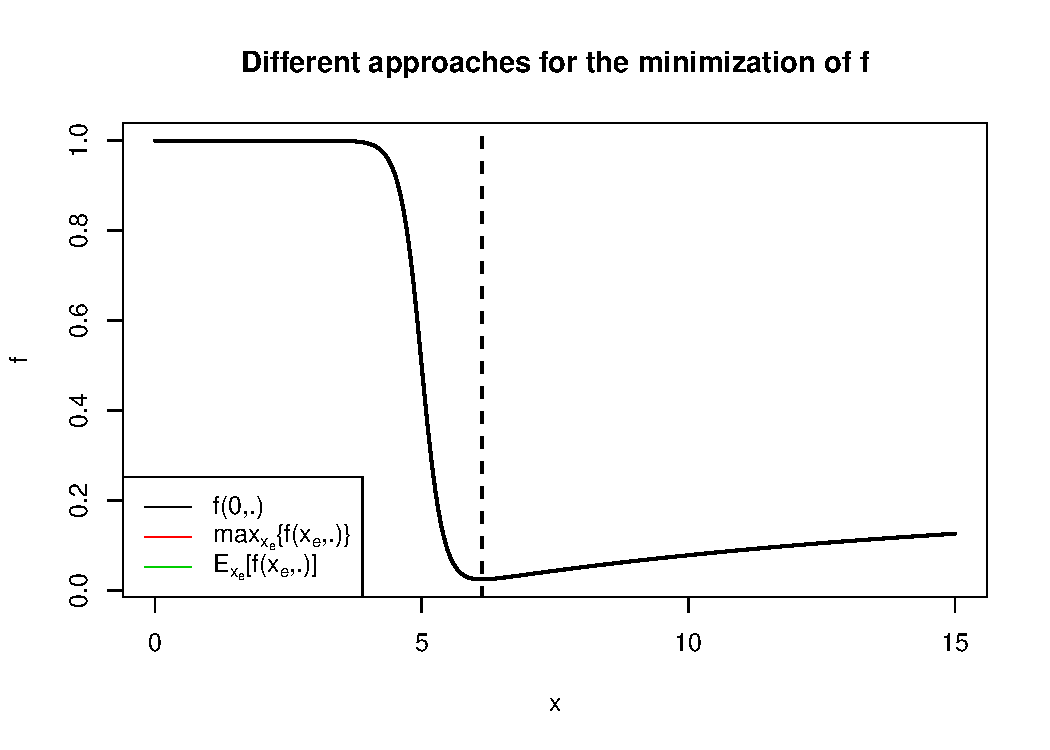
\includegraphics[scale = 0.5]{mean_worstcase_robustness1}
	\end{figure}
}
\frame{
	\frametitle{An illustration}
	$(x_e,K) \mapsto f(x_e,K) = \tilde{f}(x_e+K)$ \\ $X_e \sim \mathcal{N}(0,s^2)$ truncated on $[{-3};3]$. {\color{red}	Plot of $\max_{x_e} \{f(x_e,\cdot)\}$} \vfill
	\begin{figure}[!h]
	\centering
	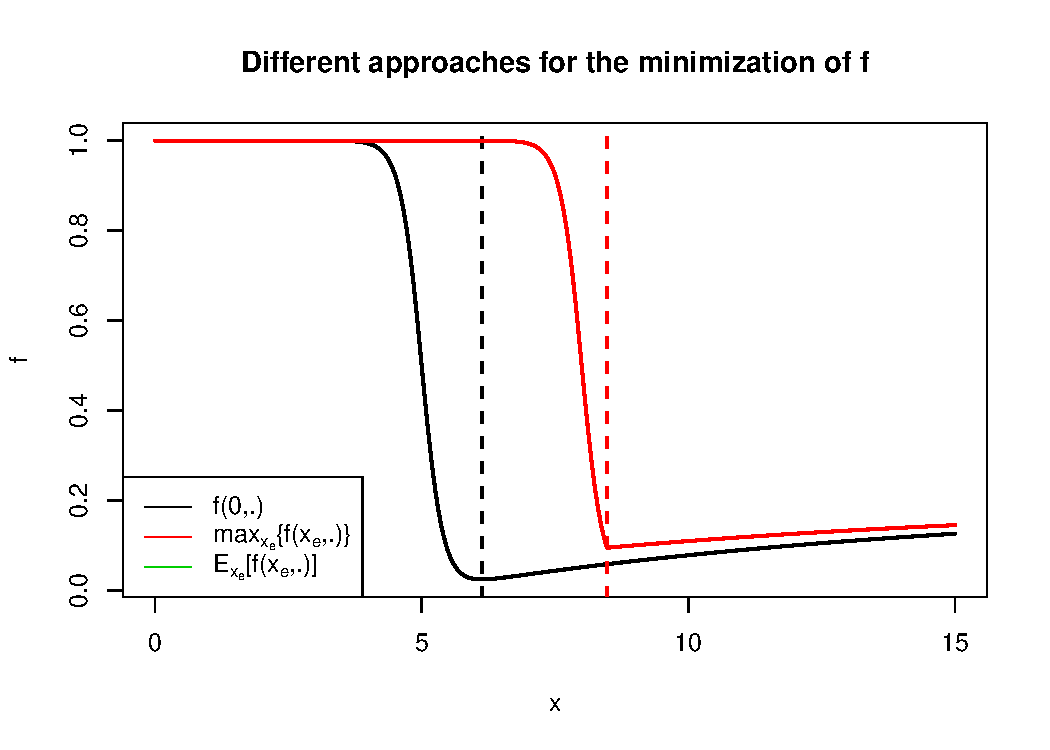
\includegraphics[scale = 0.5]{../Figures/mean_worstcase_robustness2}
	\end{figure}
}
\frame{
	\frametitle{An illustration}
	$(x_e,K) \mapsto f(x_e,K) = \tilde{f}(x_e+K)$ \\ $X_e \sim \mathcal{N}(0,s^2)$ truncated on $[{-3};3]$. {\color{green} Plot of $\Ex_{x_e}[f(x_e,\cdot)]$} \vfill
	\begin{figure}[!h]
	\centering
	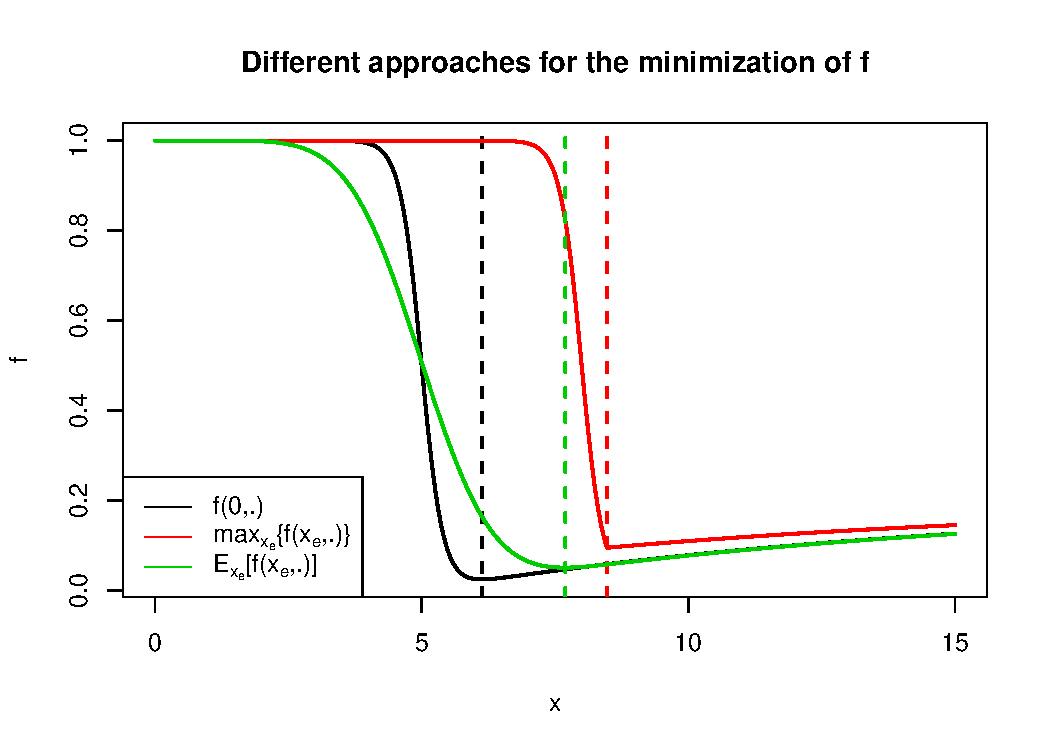
\includegraphics[scale = 0.5]{../Figures/mean_worstcase_robustness3}
	\end{figure}
}

%\subsection{Bayesian inference}
%\frame{
%\frametitle{Bayesian approach}
%Having observed $Y$, joint distribution of $(K,\bm{X}_e)$ ?
%\begin{block}{Bayes' Theorem}
%\begin{align*}
%p(K,\bm{X}_e | Y) &\propto p(Y|K,\bm{X}_e)\pi(K,\bm{X}_e) \\
%					& \propto L(K,\bm{X}_e; Y) \pi(K)\pi(\bm{X}_e)
%\end{align*}
%Estimation of the posterior distribution: computationally expensive techniques such as Markov Chain Monte Carlo.
%\end{block}
%}
\frame[t]{
\frametitle{Why surrogates?}
\begin{itemize}
\item Computer model: \alert{expensive to run}
\item $\dim \mathcal{K}$ , $\dim \mathbb{X}$ can be very large
\item Convenient way to introduce uncertainties upon $\bm{x}_e$ directly in the model
\end{itemize}
\vfill
\begin{center}
	\only<1>{\scalebox{0.9}{
\tikzstyle{block} = [rectangle, draw, fill=blue!20, 
     text centered, minimum width=1cm]
\tikzstyle{block2} = [rectangle, draw, fill=green!20, 
     text centered, , minimum width=6cm]

\tikzstyle{LHS}=[rectangle, draw, text centered]

\begin{tikzpicture}[node distance=3cm]

\node [align = center] at (0,0) (input) {Control variable \\$K \in \mathcal{K}$};
\node [align = center] at (4,1.5) (envir) {Environmental variables \\$\bm{X}_e$ random};
\node[block] at (4,0)(code){Direct Simulation};
\node[align = center] at (7,0) (output) {$W(\bm{x}_e,K)$};
\node[align = center] at (9.2,0) (jfun) {$j(\bm{x}_e,K)$};
\draw[->] (input) -- (code);
\draw[->] (envir) -- (code);
\draw[->] (code) -- (output);
\draw[->] (output) --(jfun);



\end{tikzpicture}}}	
	\only<2>{\scalebox{0.9}{
\tikzstyle{block} = [rectangle, draw, fill=blue!20, 
     text centered, minimum width=1cm]
\tikzstyle{block2} = [rectangle, draw, fill=green!20, 
     text centered, , minimum width=6cm]

\tikzstyle{LHS}=[rectangle, draw, text centered]

\begin{tikzpicture}[node distance=3cm]

\node [align = center] at (0,0) (input) {Control variable \\$K \in \mathcal{K}$};
\node [align = center] at (4,1.5) (envir) {Environmental variables \\$\bm{X}_e$ random};
\node[block] at (4,0)(code){Computer Code};
\node[align = center] at (7,0) (output) {$W(\bm{x}_e,K)$};
\node[align = center] at (9.2,0) (jfun) {$\bar{j}(\bm{x}_e,K)$};
\draw[->] (input) -- (code);
\draw[->] (envir) -- (code);
\draw[->] (code) -- (output);
\draw[->] (output) --(jfun);
\node[block2] at (5,0) (surr) {Metamodel};
\draw[->] (input) -- (surr);


\end{tikzpicture}}}
\end{center}
\vfill
}
\frame{
\frametitle{Using surrogates for optimization : adaptative sampling}
Based on kriging model $\longrightarrow$ mean and variance \\
How to choose a new point to evaluate ? 
Criterion $\kappa(\bm{x}) \longrightarrow$ "potential" of the point
\begin{equation*}
\bm{x}_{\mathrm{new}} = \argmax \kappa(\bm{x})
\end{equation*}
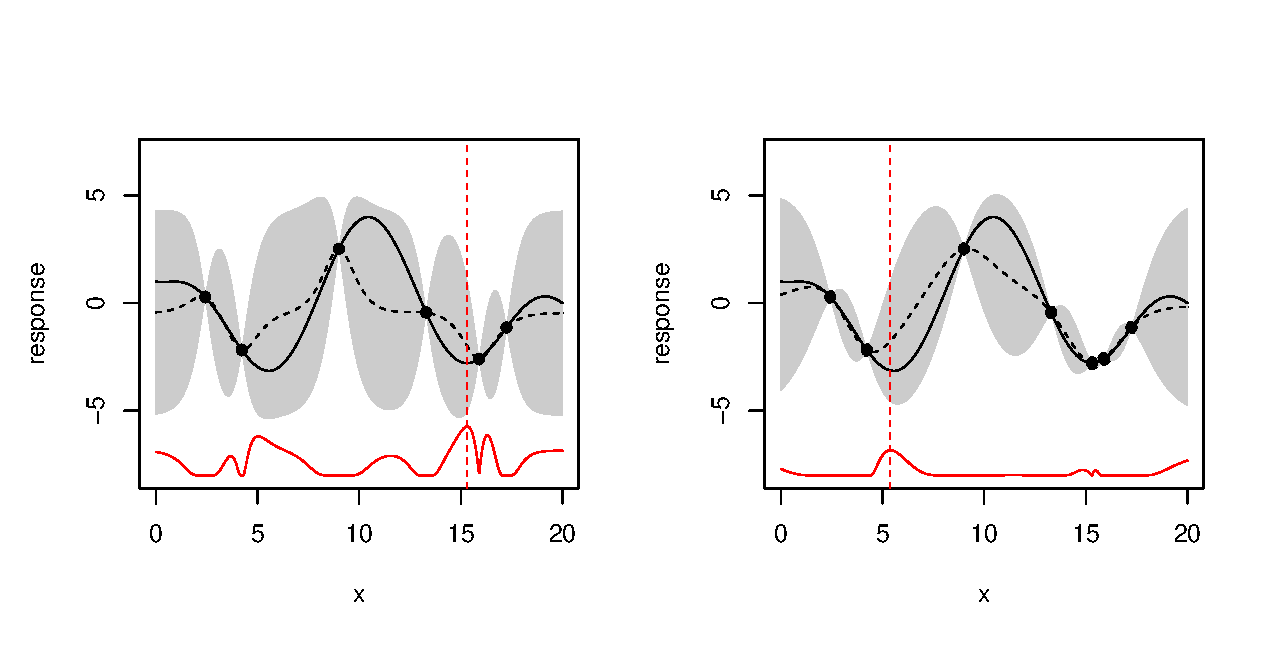
\includegraphics[width = \textwidth]{example_EGO}
}

\section{Conclusion}
\frame{
\frametitle{Conclusion}
\begin{block}{Wrapping up}
\begin{itemize}
\item Variational and bayesian approaches for this inverse problem results in different methods
\item In both case, these strategies rely heavily on surrogate models $\longrightarrow$ Kriging, Polynomial chaos
\end{itemize}
\end{block}


\begin{block}{Perspective and future work}
\begin{itemize}
\item Bayesian formulation ?
\item Cost of computer evaluations $\rightarrow$ limit the total number of runs

\item Dimensionality of the input space $\rightarrow$ reduction of the input space ?

\item How to deal with uncontrollable errors $\rightarrow$ errors between model and reality ?
\end{itemize}
\end{block}
}

\end{document}